\documentclass[12pt,xcolor=table]{beamer}
\usepackage[utf8]{inputenc}
\usepackage[T5]{fontenc}
\usepackage[vietnamese]{babel}
% --- Theme ---
\usetheme{Warsaw}
\setbeamertemplate{navigation symbols}{} % ẩn icon điều hướng cho gọn
\usepackage{appendixnumberbeamer} % đảm bảo \inserttotalframenumber hoạt động ổn
\usepackage{multirow}
\usepackage{booktabs}
% --- Gói thường dùng ---
\usepackage{graphicx}
\usepackage{xcolor}
\usepackage{colortbl}
\usepackage{tikz}
\usepackage{amsmath, amsfonts, amssymb}
\usepackage{hyperref}
\usepackage{multicol}
\usepackage{tabularx}
\usepackage{booktabs}
\allowdisplaybreaks
\setbeamertemplate{headline}{}
% --- Thông tin tiêu đề ---
\title[InstOptima]{InstOptima}
\author{Nhóm 8 CS410.Q21}
\institute[]{Trường Đại học Công nghệ Thông tin, ĐHQG-HCM\\\textit{CS410.Q21}}
\date{May 26, 2026}

% --- Footline tuỳ biến (hoạt động tốt trên Warsaw) ---
\setbeamerfont{author}{size=\footnotesize}
\setbeamertemplate{footline}{%
  \leavevmode%
  \hbox{%
    % Nửa trái
    \begin{beamercolorbox}[wd=.5\paperwidth,ht=2.5ex,dp=1ex,leftskip=1em]{author in head/foot}%
      Nhóm 8 \quad | \quad CS410.Q21 \quad | \quad TS.\;Lương Ngọc Hoàng
    \end{beamercolorbox}%
    % Nửa phải
    \begin{beamercolorbox}[wd=.5\paperwidth,ht=2.5ex,dp=1ex,center]{title in head/foot}%
      InstOptima \hfill \insertframenumber{} / \inserttotalframenumber
    \end{beamercolorbox}%
  }%
}
\graphicspath{{./}{images/7.4/}}
\begin{document}

% Trang tiêu đề
\begin{frame}
    \titlepage
\end{frame}

\begin{frame}{Thành viên nhóm}

\begin{itemize}
    \item  Ngô Phương Nam - 23520375
    \item  Phan Công Nam - 23520986
    \item  Võ Hoàng Minh - 23520961
    \item Đào Mạnh Dũng - 23520325
\end{itemize}

\end{frame}

%--------------------------------------------------------
%SLIDE 1 GIOI THIEU TASK
%--------------------------------------------------------
\section{Giới thiệu}
\begin{frame}{Mục lục}
    \setbeamercovered{dynamic}
    \tableofcontents[currentsection]
\end{frame}

\begin{frame}{Sinh văn bản dựa trên Instruction}
    \textbf{Nhiệm vụ:} Instruction (hay prompt) đóng vai trò quan trọng trong việc giúp các Mô hình Ngôn ngữ thực hiện in-context learning.
    \vspace{0.3cm}

    \textbf{Công thức hóa:} Quá trình sinh văn bản tổng quát được định nghĩa toán học như sau:
    \begin{align*}
        I &= \text{Concat}(d, e) \\
        \hat{y} &= f(x, I)
    \end{align*}
    \vspace{0.1cm}
    \begin{center}
        \textit{(trong đó $f$ là mô hình ngôn ngữ, $x$ là đầu vào mới, $\hat{y}$ là dự đoán của mô hình, $d$ là definition, và $e$ là example)}
    \end{center}
\end{frame}

%--------------------------------------------------------
%SLIDE 2 INSTRUCTION EXAMPLE
%--------------------------------------------------------
\begin{frame}{Instruction}

    \begin{block}{Ví dụ về Instruction}
        \textbf{<Definition>:} Please read customer's reviews and predict sentiments: \\
        \textbf{<Example>:} I really like this movie! Sentiment: positive \\
        Predict the sentiment: \textbf{<Input>}
    \end{block}

    \vspace{0.3cm}
    \textbf{Phân tích:}
    \begin{itemize}
        \item \textbf{Definition ($d$)} chỉ định rõ tác vụ mục tiêu cho mô hình.
        \item \textbf{Example ($e$)} cung cấp minh họa few-shot cho tác vụ.
        \item \textbf{<Input>} là vị trí đặt đầu vào của mô hình.
    \end{itemize}
\end{frame}

%--------------------------------------------------------
%SLIDE 3 MOTIVATION
%--------------------------------------------------------
\begin{frame}{Động lực nghiên cứu}
    Dù có nhiều tiến bộ gần đây, các phương pháp học dựa trên instruction hiện tại vẫn đối mặt với ba vấn đề nghiêm trọng:
    \vspace{0.5cm}
    \begin{enumerate}
        \item \textbf{Không hiệu quả:} Tìm kiếm intruction tốt rất tốn kém về mặt tính toán.
        \item \textbf{Mục tiêu tối ưu hạn hẹp:} Chỉ dựa vào độ chính xác của output mô hình.
        \item \textbf{Thiếu tính đa dạng:} Không tạo được nhiều instruction thay thế chất lượng.
    \end{enumerate}
\end{frame}

%--------------------------------------------------------
%SLIDE 4 problem 1
%--------------------------------------------------------
\begin{frame}{Vấn đề 1: Không hiệu quả}
    \begin{itemize}
        \item \textbf{Rào cản:} Văn bản là không gian tìm kiếm lớn và không khả vi.
        \item \textbf{Thất bại:} Các phương pháp chỉnh sửa và sinh văn bản tự động truyền thống cực kỳ không hiệu quả.
        \item \textbf{Kết quả:} Gần như không thể tìm kiếm toán học các instruction chất lượng cao và đa dạng bằng phương pháp tự động hiện có.
    \end{itemize}
\end{frame}

%--------------------------------------------------------
%SLIDE 5 problem 2
%--------------------------------------------------------
\begin{frame}{Vấn đề 2: Mục tiêu tối ưu hóa đơn giản}
    \begin{itemize}
        \item \textbf{Góc nhìn hạn hẹp:} Nghiên cứu hiện tại coi hiệu suất (accuracy) là tiêu chí \textit{duy nhất} đánh giá chất lượng instruction.
        \item \textbf{Những yếu tố bị bỏ qua:}
        \begin{itemize}
            \item \textbf{Length (Độ dài):} Instruction ngắn hơn giảm chi phí tính toán và thời gian huấn luyện.
            \item \textbf{Perplexity:} Perplexity thấp hơn đảm bảo văn bản tự nhiên và dễ hiểu với mô hình AI.
        \end{itemize}

    \end{itemize}
\end{frame}

%--------------------------------------------------------
%SLIDE 6 problem 3
%--------------------------------------------------------
\begin{frame}{Vấn đề 3: Thiếu tính đa dạng của Instruction}
    \begin{itemize}
        \item \textbf{Nguy cơ:} Phụ thuộc vào một prompt ``tốt nhất'' duy nhất khiến mô hình dễ bị tấn công đối kháng.
        \item \textbf{Điểm yếu:} Ngay cả khi instruction bị nhiễu nhẹ, như thay thế từ đồng nghĩa, cũng có thể gây giảm hiệu suất đột ngột.
    \end{itemize}
\end{frame}

%--------------------------------------------------------
%SLIDE 7 gioi thieu InstOptima
%--------------------------------------------------------
\section{InstOptima}
\begin{frame}{Mục lục}
    \setbeamercovered{dynamic}
    \tableofcontents[currentsection]
\end{frame}

\begin{frame}{InstOptima}
    \textbf{InstOptima} xem việc sinh instruction như một bài toán tối ưu hóa đa mục tiêu tiến hóa.
    \vspace{0.3cm}
    \begin{itemize}
        \item \textbf{Giải quyết không hiệu quả:} Sử dụng ChatGPT để mô phỏng các toán tử di truyền (mutation và crossover) trên instruction.
        \item \textbf{Giải quyết mục tiêu hạn hẹp:} Kết hợp đồng thời ba mục tiêu: Performance, Length và Perplexity.
        \item \textbf{Giải quyết thiếu đa dạng:} Dùng thuật toán NSGA-II để thu được Pareto front giúp đa dạng các instruction chất lượng cao.
    \end{itemize}
\end{frame}

%--------------------------------------------------------
%SLIDE Quy trinh tong quat
%--------------------------------------------------------
\begin{frame}{Quy trình hoạt động của InstOptima}

\begin{figure}
    \centering
    \includegraphics[width=\textwidth, height=0.75\textheight, keepaspectratio]{IMAGES/IMAGE1-CS410.png}
\end{figure}

\end{frame}




%--------------------------------------------------------
%SLIDE 10 Objectives
%--------------------------------------------------------
\begin{frame}{Các mục tiêu tối ưu hóa}

    \begin{block}{Ba mục tiêu tối ưu F = (m,l,r)}
        \begin{enumerate}
            \item \textbf{Performance (m):} Đánh giá bằng các chỉ số accuracy, F1, precision và recall.
            \vspace{0.2cm}
            \item \textbf{Length (l):} Đo bằng số ký tự, đảm bảo so sánh công bằng bất kể chiến lược tokenization của mô hình.
            \vspace{0.2cm}
            \item \textbf{Perplexity (r):} Đo bằng mô hình RoBERTa. Perplexity thấp hơn đảm bảo instruction tự nhiên và dễ hiểu với mô hình ngôn ngữ.
        \end{enumerate}
    \end{block}
\end{frame}

%--------------------------------------------------------
%SLIDE Cong thuc 3 muc tieu
%--------------------------------------------------------
\begin{frame}{Công thức của 3 mục tiêu}
    InstOptima xem mỗi instruction $I = \text{Concat}(d,e)$ là một cá thể, và \textbf{cực tiểu hóa} đồng thời bộ ba $F = (m, l, r)$:

    \begin{align*}
        m &= \dfrac{1}{\text{Accuracy} + \text{Precision} + \text{Recall} + \text{F1}} \\[4pt]
        l &= \big|\,\text{Concat}(d, e)\,\big| \quad \text{(số ký tự của instruction)} \\[4pt]
        r &= \exp\!\left(\dfrac{\mathcal{L}_{\text{RoBERTa-MLM}}(I)}{|I|}\right)
    \end{align*}

    \begin{itemize}
        \item $m$: \textbf{nghịch đảo} tổng 4 chỉ số hiệu suất -- accuracy/F1/precision/recall \textit{càng cao} thì $m$ \textit{càng thấp} (càng tốt).
        \item $l$: số ký tự của $I$, không phụ thuộc tokenizer.
        \item $r$: perplexity của $I$ tính bằng masked-LM loss của RoBERTa.
    \end{itemize}
\end{frame}

%--------------------------------------------------------
%SLIDE Su doi lap giua 3 muc tieu
%--------------------------------------------------------
\begin{frame}{Sự đối lập (trade-off) giữa các mục tiêu}
    \begin{itemize}
        \item \textbf{Length $\leftrightarrow$ Perplexity:} Instruction dài, có giải thích và ví dụ minh họa tự nhiên thường \textit{dễ hiểu hơn} với mô hình ngôn ngữ (perplexity $r$ thấp), nhưng tăng chi phí tính toán/huấn luyện ($l$ tăng). Ngược lại, instruction ngắn gọn giảm $l$ nhưng có thể kém tự nhiên hơn (tăng $r$).
        \vspace{0.2cm}
        \item \textbf{Performance $\leftrightarrow$ Length:} Để giảm $m$ (tăng accuracy/F1), instruction thường cần thêm chi tiết, ràng buộc, ví dụ $\to$ tăng $l$. Rút ngắn instruction có thể làm mất thông tin cần thiết, làm tăng $m$.
        \vspace{0.2cm}
        \item \textbf{Performance $\leftrightarrow$ Perplexity:} Một instruction ``tự nhiên'' (giảm $r$) đôi khi thiếu các chỉ dẫn đặc thù cho tác vụ, khiến $m$ khó giảm thêm.
    \end{itemize}
\end{frame}

%--------------------------------------------------------
%SLIDE gioi thieu Operators
%--------------------------------------------------------
\begin{frame}{Các toán tử (Operators)}
    \begin{itemize}
        \item \textbf{Mục đích:} Để xử lý không gian tìm kiếm văn bản lớn và không khả vi, InstOptima dùng ChatGPT để chỉnh sửa văn bản.
        \item \textbf{Prompt cố định ($\tilde{P}$):} Thuật toán sử dụng các prompt ẩn được định nghĩa sẵn để điều hướng hành vi của ChatGPT.
        \item \textbf{Bốn toán tử cốt lõi:}
        \begin{enumerate}
            \item Definition Mutation ($\tilde{P}_{dm}$)
            \item Definition Crossover ($\tilde{P}_{dc}$)
            \item Example Mutation ($\tilde{P}_{em}$)
            \item Example Crossover ($\tilde{P}_{ec}$)
        \end{enumerate}
    \end{itemize}
\end{frame}

%--------------------------------------------------------
%SLIDE 11 Objective-Guided Instruction
%--------------------------------------------------------
\begin{frame}{Instruction Operator hướng dẫn bởi mục tiêu}
    \begin{itemize}
        \item \textbf{Cơ chế:} InstOptima truyền trực tiếp các điểm fitness $F = (m, l, r)$ (performance, length, perplexity) vào prompt gửi cho ChatGPT.
        \item \textbf{Ví dụ:} ``Please refer to the objective values: ($d_1, F_1$), ($d_2, F_2$)''.
        \item \textbf{Ý nghĩa:} Đây là vòng phản hồi tự động -- ChatGPT tự quyết định nhấn mạnh hay giảm bớt các phần của instruction dựa trên điểm số toán học hiện tại.
    \end{itemize}
\end{frame}

%--------------------------------------------------------
%SLIDE 8 Operator 1
%--------------------------------------------------------

\begin{frame}{Definition Mutation}
    \begin{quote}
        ``I want you to be a professional prompt engineer. Now I am working on the multi-objective evolutionary
prompt optimization, and I need your help to design and optimize the template prompt. Here I give
you an example template prompt, please understand the meaning of the prompt and modify it. \textcolor{green!50!black}{Given
the minimization objectives}, please be creative and output the paraphrased or mutated prompt. Please
remove Minimization objectives in the output: \textcolor{green!50!black}{(``Please read customer's reviews and predict sentiments:'', (0.32, 101, 1.25))}''
    \end{quote}
\end{frame}
\begin{frame}{Definition Mutation}
    \begin{block}{Quá trình}
        \vspace{-0.5cm}
        \begin{align*}
            \hat{d}_{dm} &= \text{ChatGPT}(\text{Concat}(\tilde{P}_{dm}, d_1, F_1)) \\
            \hat{I} &= \text{Concat}(\hat{d}_{dm}, e_1)
        \end{align*}
    \end{block}
    \vspace{0.3cm}
    \begin{block}{Ví dụ: <Input> = $(d_1, F_1)$ gửi cho ChatGPT}
        \footnotesize
        $d_1$: ``Please read customer's reviews and predict sentiments:'' \\
        $F_1=(m_1, l_1, r_1) = (0.32,\ 101,\ 1.25)$ \\[3pt]
        $\Rightarrow \hat{d}_{dm}$: ``Let's classify the customers' sentiments.''\\
        $e_1$: ``I really like this movie! Sentiment: positive'' \\

        \vspace{2pt}
        {$\hat{l} = |\text{Concat}(\hat{d_{dm}}, e_1)$ = ``Let's classify the customers' sentiments. I really like this movie! Sentiment: positive''}
    \end{block}
\end{frame}

%--------------------------------------------------------
%SLIDE 9 Operator 2
%--------------------------------------------------------
\begin{frame}{Definition Crossover}
    \begin{quote}
        ``I want you to be a professional prompt engineer. Now I am working on the multi-objective evolutionary prompt optimization for sentiment analysis, and I need your help to design and optimize the template prompt. Here I give you two template prompts, please understand the meaning of the two prompts and crossover them into a new prompt. Given the minimization objectives, please be creative and output the generated new prompt based on the two examples. Please remove Minimization objectives in the output: \textcolor{green!50!black}{(``Please read customer's reviews and predict sentiments:'', (0.32, 101, 1.25)), (``Analyze the sentiment expressed in the review:'', (0.35, 46, 1.42))}''
    \end{quote}
\end{frame}
\begin{frame}{Definition Crossover}
    \begin{block}{Quá trình}
        \vspace{-0.5cm}
        \begin{align*}
            \hat{d}_{dc} &= \text{ChatGPT}(\text{Concat}(\tilde{P}_{dc}, d_1, F_1, d_2, F_2)) \\
            \hat{I} &= \text{Concat}(\hat{d}_{dc}, e_1)
        \end{align*}
    \end{block}
\end{frame}
%--------------------------------------------------------
%SLIDE Pseudocode
%--------------------------------------------------------
\begin{frame}{Quy trình hoạt động của InstOptima}

\begin{figure}
    \centering
    \includegraphics[width=\textwidth, height=0.75\textheight, keepaspectratio]{IMAGES/IMAGE2-CS410.png}
\end{figure}

\end{frame}




%--------------------------------------------------------
%SLIDE Thuc nghiem
%--------------------------------------------------------
\section{Thực nghiệm}

\begin{frame}{Mục lục}
    \setbeamercovered{dynamic}
    \tableofcontents[currentsection]
\end{frame}

\begin{frame}{Thiết kế thực nghiệm}
    \textbf{Mục tiêu:} Đánh giá xem InstOptima có thể tự động tối ưu hóa instruction hiệu quả hơn các phương pháp thông thường thông qua tối ưu hóa tiến hóa đa mục tiêu hay không.
    \vspace{0.5cm}

    \textbf{Các điểm kiểm chứng chính:}
    \begin{itemize}
        \vspace{0.1cm}
        \item Instruction được tối ưu có cải thiện hiệu suất mô hình NLP không?
        \vspace{0.1cm}
        \item Các instruction được sinh ra có chất lượng cao và đa dạng không?
    \end{itemize}
\end{frame}

%--------------------------------------------------------
%SLIDE Dataset
%--------------------------------------------------------
\begin{frame}{Bộ dữ liệu}
    InstOptima được đánh giá trên 3 bộ dữ liệu benchmark thuộc 3 nhóm tác vụ NLP để kiểm tra khả năng tổng quát hóa:
    \vspace{0.3cm}
    \begin{itemize}
        \item \textbf{Aspect-Based Sentiment Analysis (ABSA):} Laptop14
        \item \textbf{Text Classification (TC):} SST2
        \item \textbf{Natural Language Inference (NLI):} SNLI
    \end{itemize}
    \vspace{0.3cm}

    \begin{block}{Quy mô thực nghiệm}
        Để giảm chi phí tính toán trong quá trình tiến hóa, mỗi bộ dữ liệu sử dụng chính xác: \textbf{1000} mẫu huấn luyện, \textbf{1000} mẫu kiểm định, và \textbf{1000} mẫu kiểm tra.
    \end{block}
\end{frame}

%--------------------------------------------------------
%SLIDE Models
%--------------------------------------------------------
\begin{frame}{Mô hình và đánh giá}
    \small
    Các mô hình khác nhau được phân công vai trò cụ thể trong framework:
    \vspace{0.1cm}
    \begin{itemize}
        \item \textbf{Toán tử LLM để lai ghép và đột biến (ChatGPT):} Xử lý toàn bộ quá trình tiến hóa ngữ nghĩa của instruction (Definition/Example Mutation và Crossover).
        \vspace{0.05cm}
        \item \textbf{Tính Performance instruction (FlanT5-base):} Với mỗi instruction, gắn instruction vào toàn bộ input của mẫu dữ liệu của tập train rồi thực hiện finetune FlanT5 trên các cặp (instruction + input, output) sau đó đem đi đánh giá trên tập test để tính các metrics, từ đây tính được mục tiêu performance.
        \vspace{0.05cm}
        \item \textbf{Tính Perplexity cho instruction (RoBERTa):} Đo độ phức tạp của instruction (đo bằng model RoBERTa). Perplexity thấp hơn cho thấy instruction dễ hiểu hơn với mô hình ngôn ngữ.
    \end{itemize}
\end{frame}

%--------------------------------------------------------
%SLIDE Pipeline thuc nghiem
%--------------------------------------------------------
\begin{frame}{Pipeline tính điểm 3 mục tiêu của một instruction}
    Với \textbf{mỗi instruction} $I=\text{Concat}(d,e)$ trong quần thể, một vòng đánh giá $F=(m,l,r)$ gồm:

    \begin{enumerate}
        \item \textbf{Gắn instruction vào dữ liệu:} Chèn $I$ vào trước mỗi mẫu của tập train (1000 mẫu) và tập test (1000 mẫu).
        \vspace{0.15cm}
        \item \textbf{Fine-tune FlanT5-base:} Huấn luyện trên tập train đã gắn $I$ trong 3 epochs, learning rate $5{\times}10^{-5}$, batch size 16.
        \vspace{0.15cm}
        \item \textbf{Inference trên tập test:} Mô hình vừa fine-tune sinh nhãn dự đoán cho 1000 mẫu test.
        \vspace{0.15cm}
        \item \textbf{Tính metrics:} So khớp dự đoán với nhãn thật $\to$ Accuracy, Precision, Recall, F1 (macro).
        \vspace{0.15cm}
        \item \textbf{Tính 3 mục tiêu:} $m$ từ metrics ở bước 4; $l$ = số ký tự của $I$; $r$ = perplexity của $I$ (RoBERTa).
    \end{enumerate}
\end{frame}

\begin{frame}{Pipeline tính 3 mục tiêu -- Ví dụ cụ thể (Laptop14)}
    \begin{block}{Sau khi fine-tune FlanT5-base \& đánh giá trên 1000 mẫu test}
        Accuracy $= 0.8798$, \quad Precision $= 0.7435$, \quad Recall $= 0.7411$, \quad F1 $= 0.7391$
    \end{block}
    \vspace{-0.3cm}
    \begin{align*}
        m &= \dfrac{1}{0.8798+0.7435+0.7411+0.7391} = \dfrac{1}{3.1035} \approx 0.3222 \\
        l &= 772 \ \text{(ký tự của } I=\text{Concat}(d,e)\text{)}\\
        r &= 1.0681 \ \text{(perplexity từ RoBERTa)}
    \end{align*}
    \vspace{-0.4cm}
    \begin{block}{Vai trò của $F=(m,l,r)$}
        \begin{itemize}
            \item Dùng để \textbf{xếp hạng} cá thể bằng non-dominated sorting (NSGA-II).
            \item Là \textbf{input} cho các toán tử lai ghép/đột biến ở thế hệ tiếp theo (objective-guided).
        \end{itemize}
    \end{block}
\end{frame}

%--------------------------------------------------------
%SLIDE Environment
%--------------------------------------------------------
\begin{frame}{Cấu hình tối ưu hóa và môi trường}
    \begin{itemize}
        \item \textbf{Thuật toán tối ưu hóa:} NSGA-II
        \item \textbf{Mục tiêu:} Performance, Instruction Length và Perplexity
        \item \textbf{Cấu hình tiến hóa:} Quần thể = 30, Số thế hệ = 10.
        \item \textbf{Cấu hình Fine-Tuning:} Learning Rate = $5 \times 10^{-5}$, Batch Size = 16, Epochs = 3.
    \end{itemize}
    \vspace{0.2cm}

    \begin{block}{Môi trường triển khai}
        \begin{itemize}
            \item \textbf{Frameworks:} PyTorch 2.0.0, Transformers 4.28.0
            \item \textbf{Phần cứng:} GPU RTX 3090 24gb VRAM
        \end{itemize}
    \end{block}
\end{frame}

%--------------------------------------------------------
%SLIDE Baseline
%--------------------------------------------------------
\begin{frame}{Phương pháp so sánh}
    Để đánh giá chính xác hiệu quả, InstOptima được so sánh với hai baseline:
    \vspace{0.3cm}
    \begin{enumerate}
        \item \textbf{RanInstruct (Instruction ngẫu nhiên):}
        \begin{itemize}
            \item Sinh ngẫu nhiên 5 instruction bằng ChatGPT.
            \item \textit{Mục đích:} Kiểm tra xem quá trình tối ưu hóa toán học có quan trọng hơn việc đơn giản yêu cầu LLM sinh prompt ngẫu nhiên không.
        \end{itemize}
        \vspace{0.3cm}
        \item \textbf{NoInstruct (Không có Instruction):}
        \begin{itemize}
            \item Đánh giá mô hình khi không có instruction nào.
            \item \textit{Mục đích:} Kiểm tra xem instruction có thực sự cần thiết cho tác vụ sinh văn bản không.
        \end{itemize}
    \end{enumerate}
\end{frame}

%--------------------------------------------------------
% SLIDE: Kết quả - So sánh hiệu suất (Table 1)
%--------------------------------------------------------
\begin{frame}{So sánh hiệu suất}
\resizebox{\textwidth}{!}{%
\setlength{\tabcolsep}{6pt}%
\begin{tabular}{|l|l|c|c|c|c|c|c|c|}
\hline
\rowcolor{gray!40} \textbf{Dataset} & \textbf{Phương pháp} & \textbf{Accuracy} & \textbf{Precision} & \textbf{Recall} & \textbf{F1} & \textbf{Avg} & \textbf{Length} & \textbf{Perplexity} \\
\hline
\rowcolor{blue!15} Laptop14 & NoInstruct & 0.8689 & 0.7384 & 0.7466 & 0.7394 & 0.7733 & 0.0000 & 2.7280 \\
\hline
\rowcolor{green!15} Laptop14 & RanInstruct & $0.8645{\pm}.0017$ & $0.7206{\pm}.0068$ & $0.7332{\pm}.0062$ & $0.7244{\pm}.0063$ & $0.7607{\pm}.0052$ & $370.6{\pm}21.7$ & $1.1485{\pm}.0090$ \\
\hline
\rowcolor{red!12} Laptop14 & \textbf{InstOptima} & $\mathbf{0.8798}{\pm}.0038$ & $\mathbf{0.7435}{\pm}.0105$ & $0.7411{\pm}.0109$ & $0.7391{\pm}.0106$ & $\mathbf{0.7759}{\pm}.0087$ & $772.3{\pm}221.5$ & $\mathbf{1.0681}{\pm}.0154$ \\
\hline
\rowcolor{blue!15} SST2 & NoInstruct & 0.9289 & 0.9290 & 0.9288 & 0.9289 & 0.9289 & 0.0000 & 2.7109 \\
\hline
\rowcolor{green!15} SST2 & RanInstruct & $0.9275{\pm}.0011$ & $0.9277{\pm}.0013$ & $0.9274{\pm}.0010$ & $0.9275{\pm}.0011$ & $0.9275{\pm}.0011$ & $272.6{\pm}7.9$ & $1.1707{\pm}.0131$ \\
\hline
\rowcolor{red!12} SST2 & \textbf{InstOptima} & $\mathbf{0.9307}{\pm}.0028$ & $\mathbf{0.9308}{\pm}.0028$ & $\mathbf{0.9307}{\pm}.0029$ & $\mathbf{0.9306}{\pm}.0028$ & $\mathbf{0.9307}{\pm}.0028$ & $426.4{\pm}88.3$ & $\mathbf{1.1155}{\pm}.0170$ \\
\hline
\rowcolor{blue!15} SNLI & NoInstruct & 0.8680 & 0.8738 & 0.8685 & 0.8691 & 0.8699 & 0.0000 & 2.7109 \\
\hline
\rowcolor{green!15} SNLI & RanInstruct & $0.8706{\pm}.0025$ & $0.8715{\pm}.0019$ & $0.8706{\pm}.0023$ & $0.8705{\pm}.0022$ & $0.8708{\pm}.0021$ & $315.2{\pm}7.3$ & $1.1487{\pm}.0073$ \\
\hline
\rowcolor{red!12} SNLI & \textbf{InstOptima} & $\mathbf{0.8736}{\pm}.0056$ & $\mathbf{0.8740}{\pm}.0054$ & $\mathbf{0.8733}{\pm}.0056$ & $\mathbf{0.8730}{\pm}.0059$ & $\mathbf{0.8735}{\pm}.0056$ & $461.5{\pm}116.9$ & $\mathbf{1.0966}{\pm}.0181$ \\
\hline
\end{tabular}%
}
 \begin{itemize}
        \item \textbf{InstOptima vượt RanInstruct và NoInstruct} trên cả 3 dataset về tất cả metrics.
        \item \textbf{Laptop14 \& SST2}: InstOptima là phương pháp \textit{duy nhất} vượt NoInstruct -- RanInstruct còn thấp hơn cả NoInstruct, cho thấy instruction ngẫu nhiên có thể \textit{gây hại}.
        \item \textbf{SNLI}: cả hai phương pháp đều vượt NoInstruct -- instruction (dù ngẫu nhiên) vẫn có ích trên tác vụ NLI.
    \end{itemize}
\end{frame}

\begin{frame}{So sánh hiệu suất}
    \begin{block}{Kết luận}
        Tối ưu hóa tiến hóa đa mục tiêu giúp cải thiện chất lượng instruction so với lựa chọn ngẫu nhiên; bản thân instruction cũng đóng vai trò quan trọng, đặc biệt ở các tác vụ suy diễn phức tạp như NLI.
    \end{block}
\end{frame}

%--------------------------------------------------------
% SLIDE: Kết quả - Trajectory (Figure 2)
%--------------------------------------------------------
\begin{frame}{Trajectory qua các thế hệ}
\begin{figure}
    \centering
    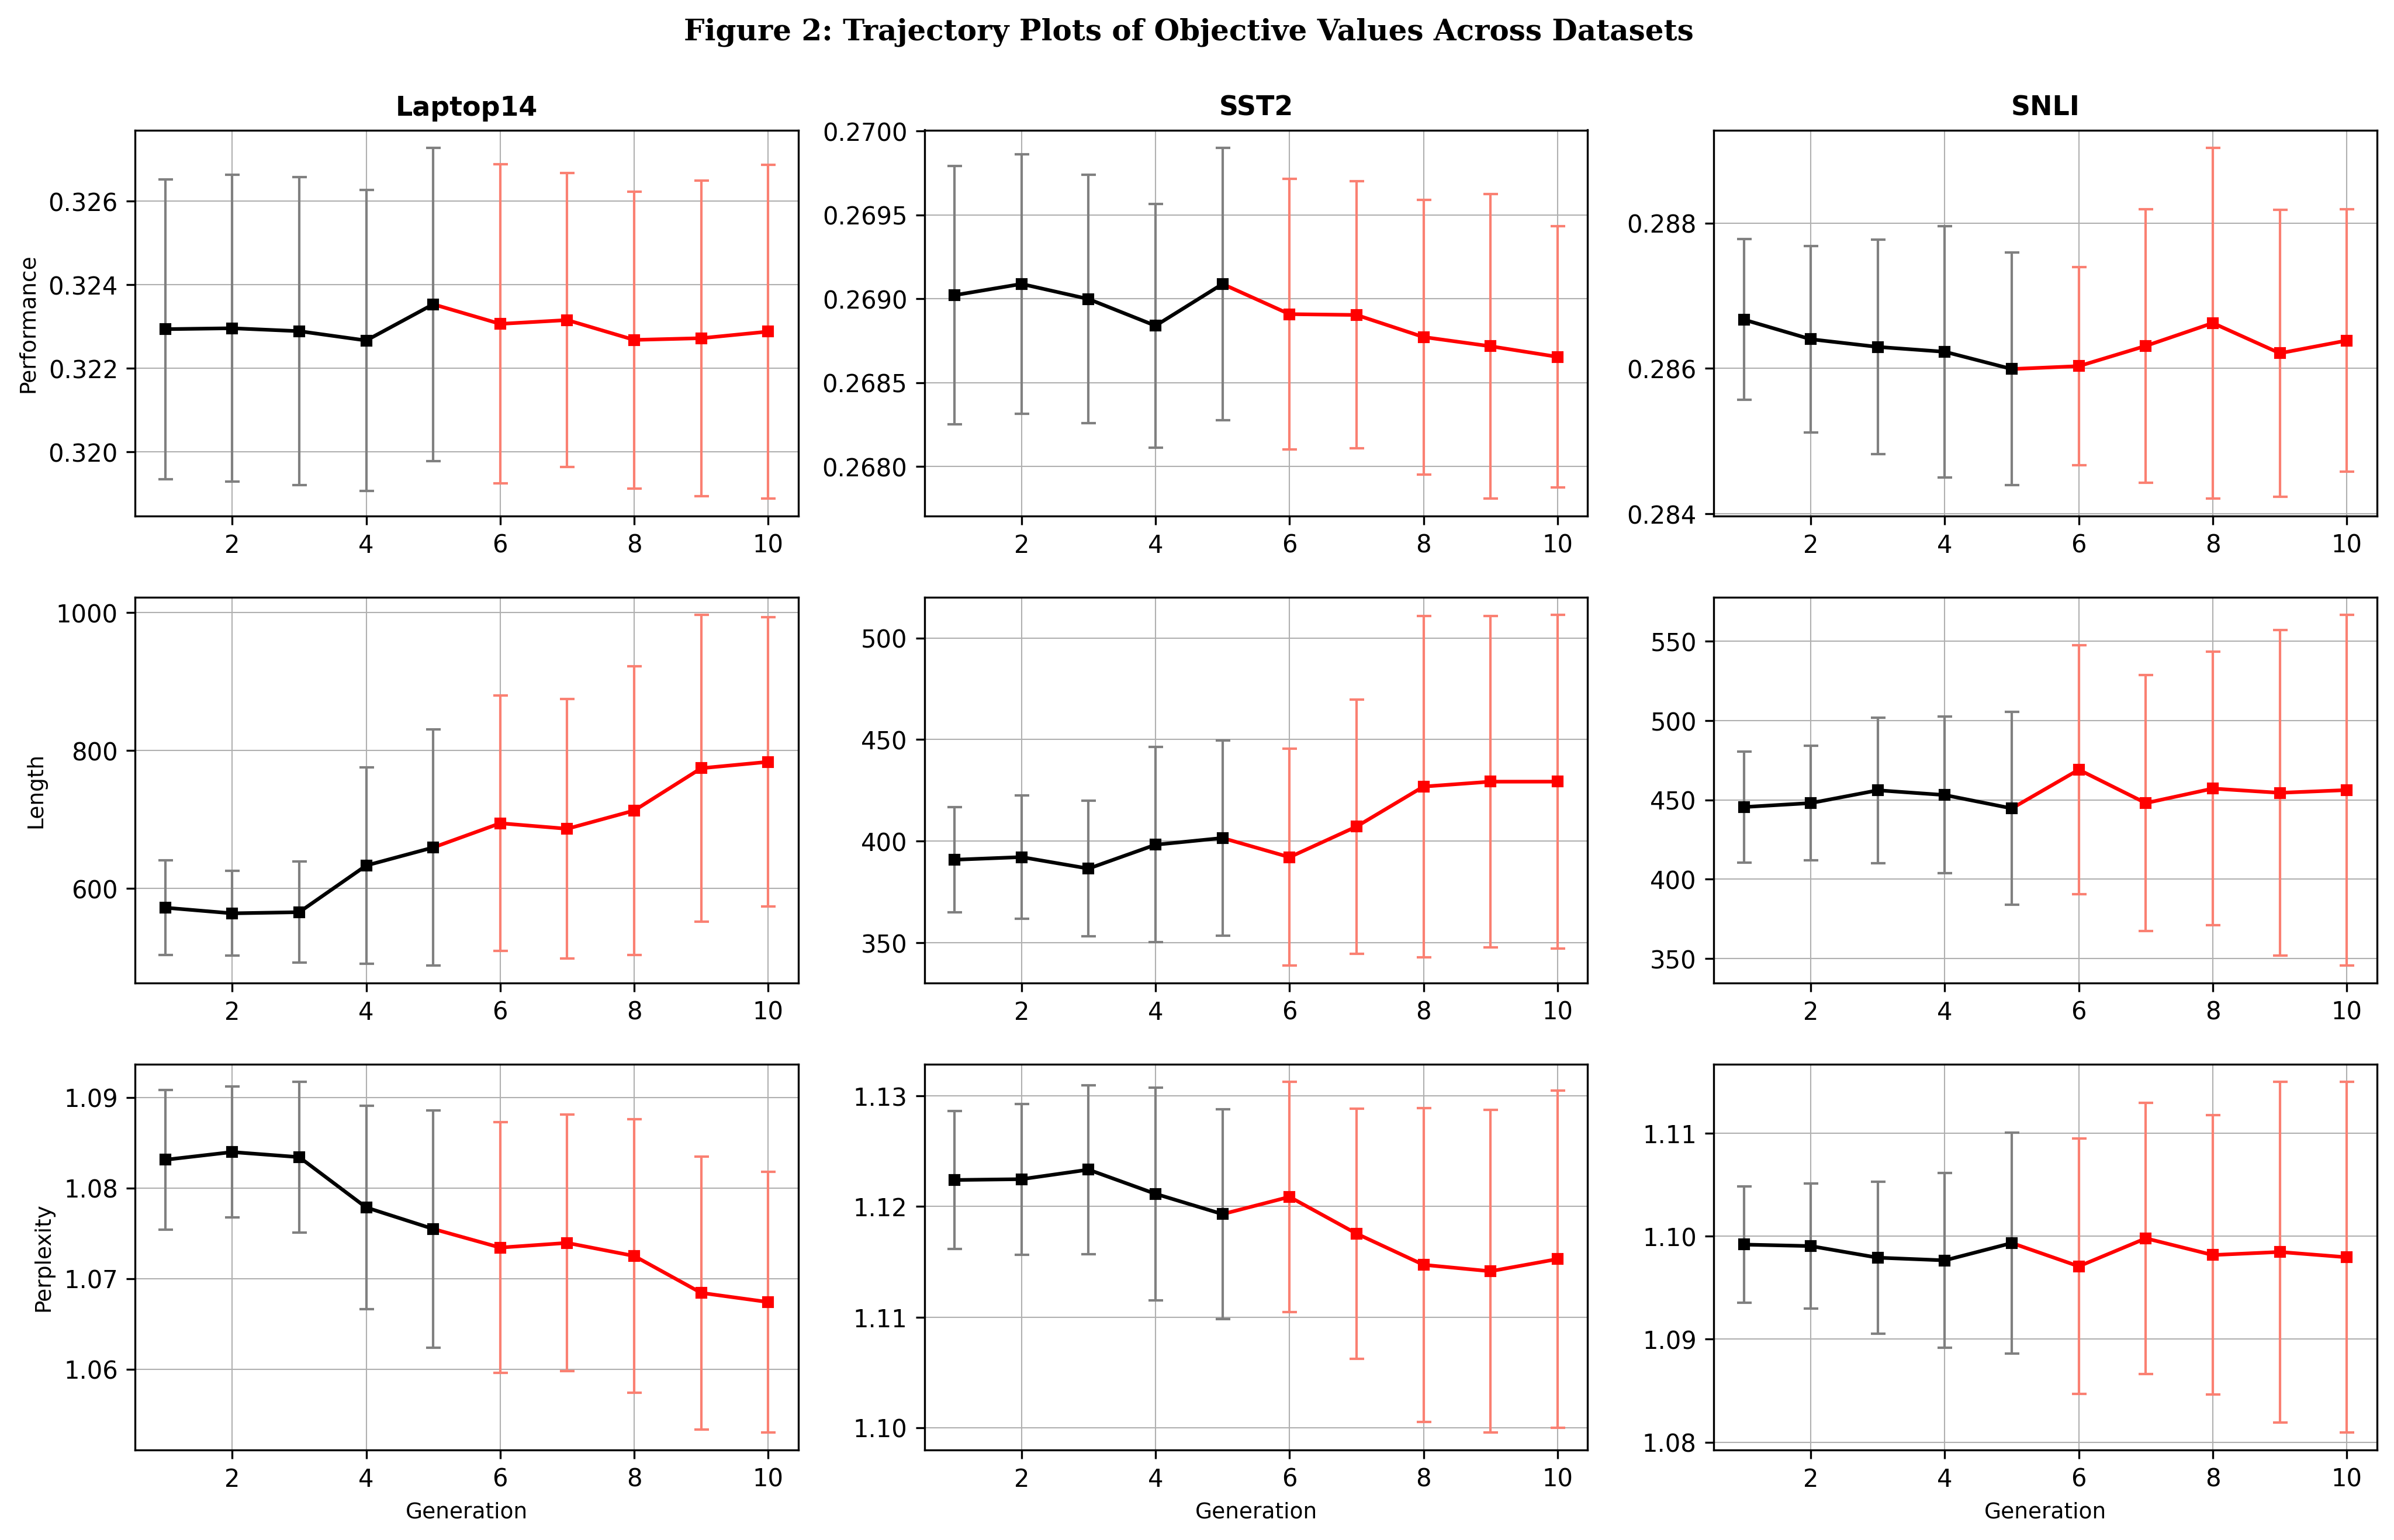
\includegraphics[width=\textwidth, height=0.75\textheight, keepaspectratio]{paper_fig2_trajectory.png}
\end{figure}
\end{frame}

\begin{frame}{Trajectory qua các thế hệ}
    \begin{block}{Kết luận}
        NSGA-II cân bằng được các mục tiêu xung đột nhau: duy trì hiệu suất trong khi liên tục cải thiện perplexity, cho thấy quá trình tiến hóa instruction là có định hướng và có ý nghĩa.
    \end{block}
\end{frame}

%--------------------------------------------------------
% SLIDE: Kết quả - Pareto Front (Figure 3)
%--------------------------------------------------------
\begin{frame}{Pareto Front}
\begin{figure}
    \centering
    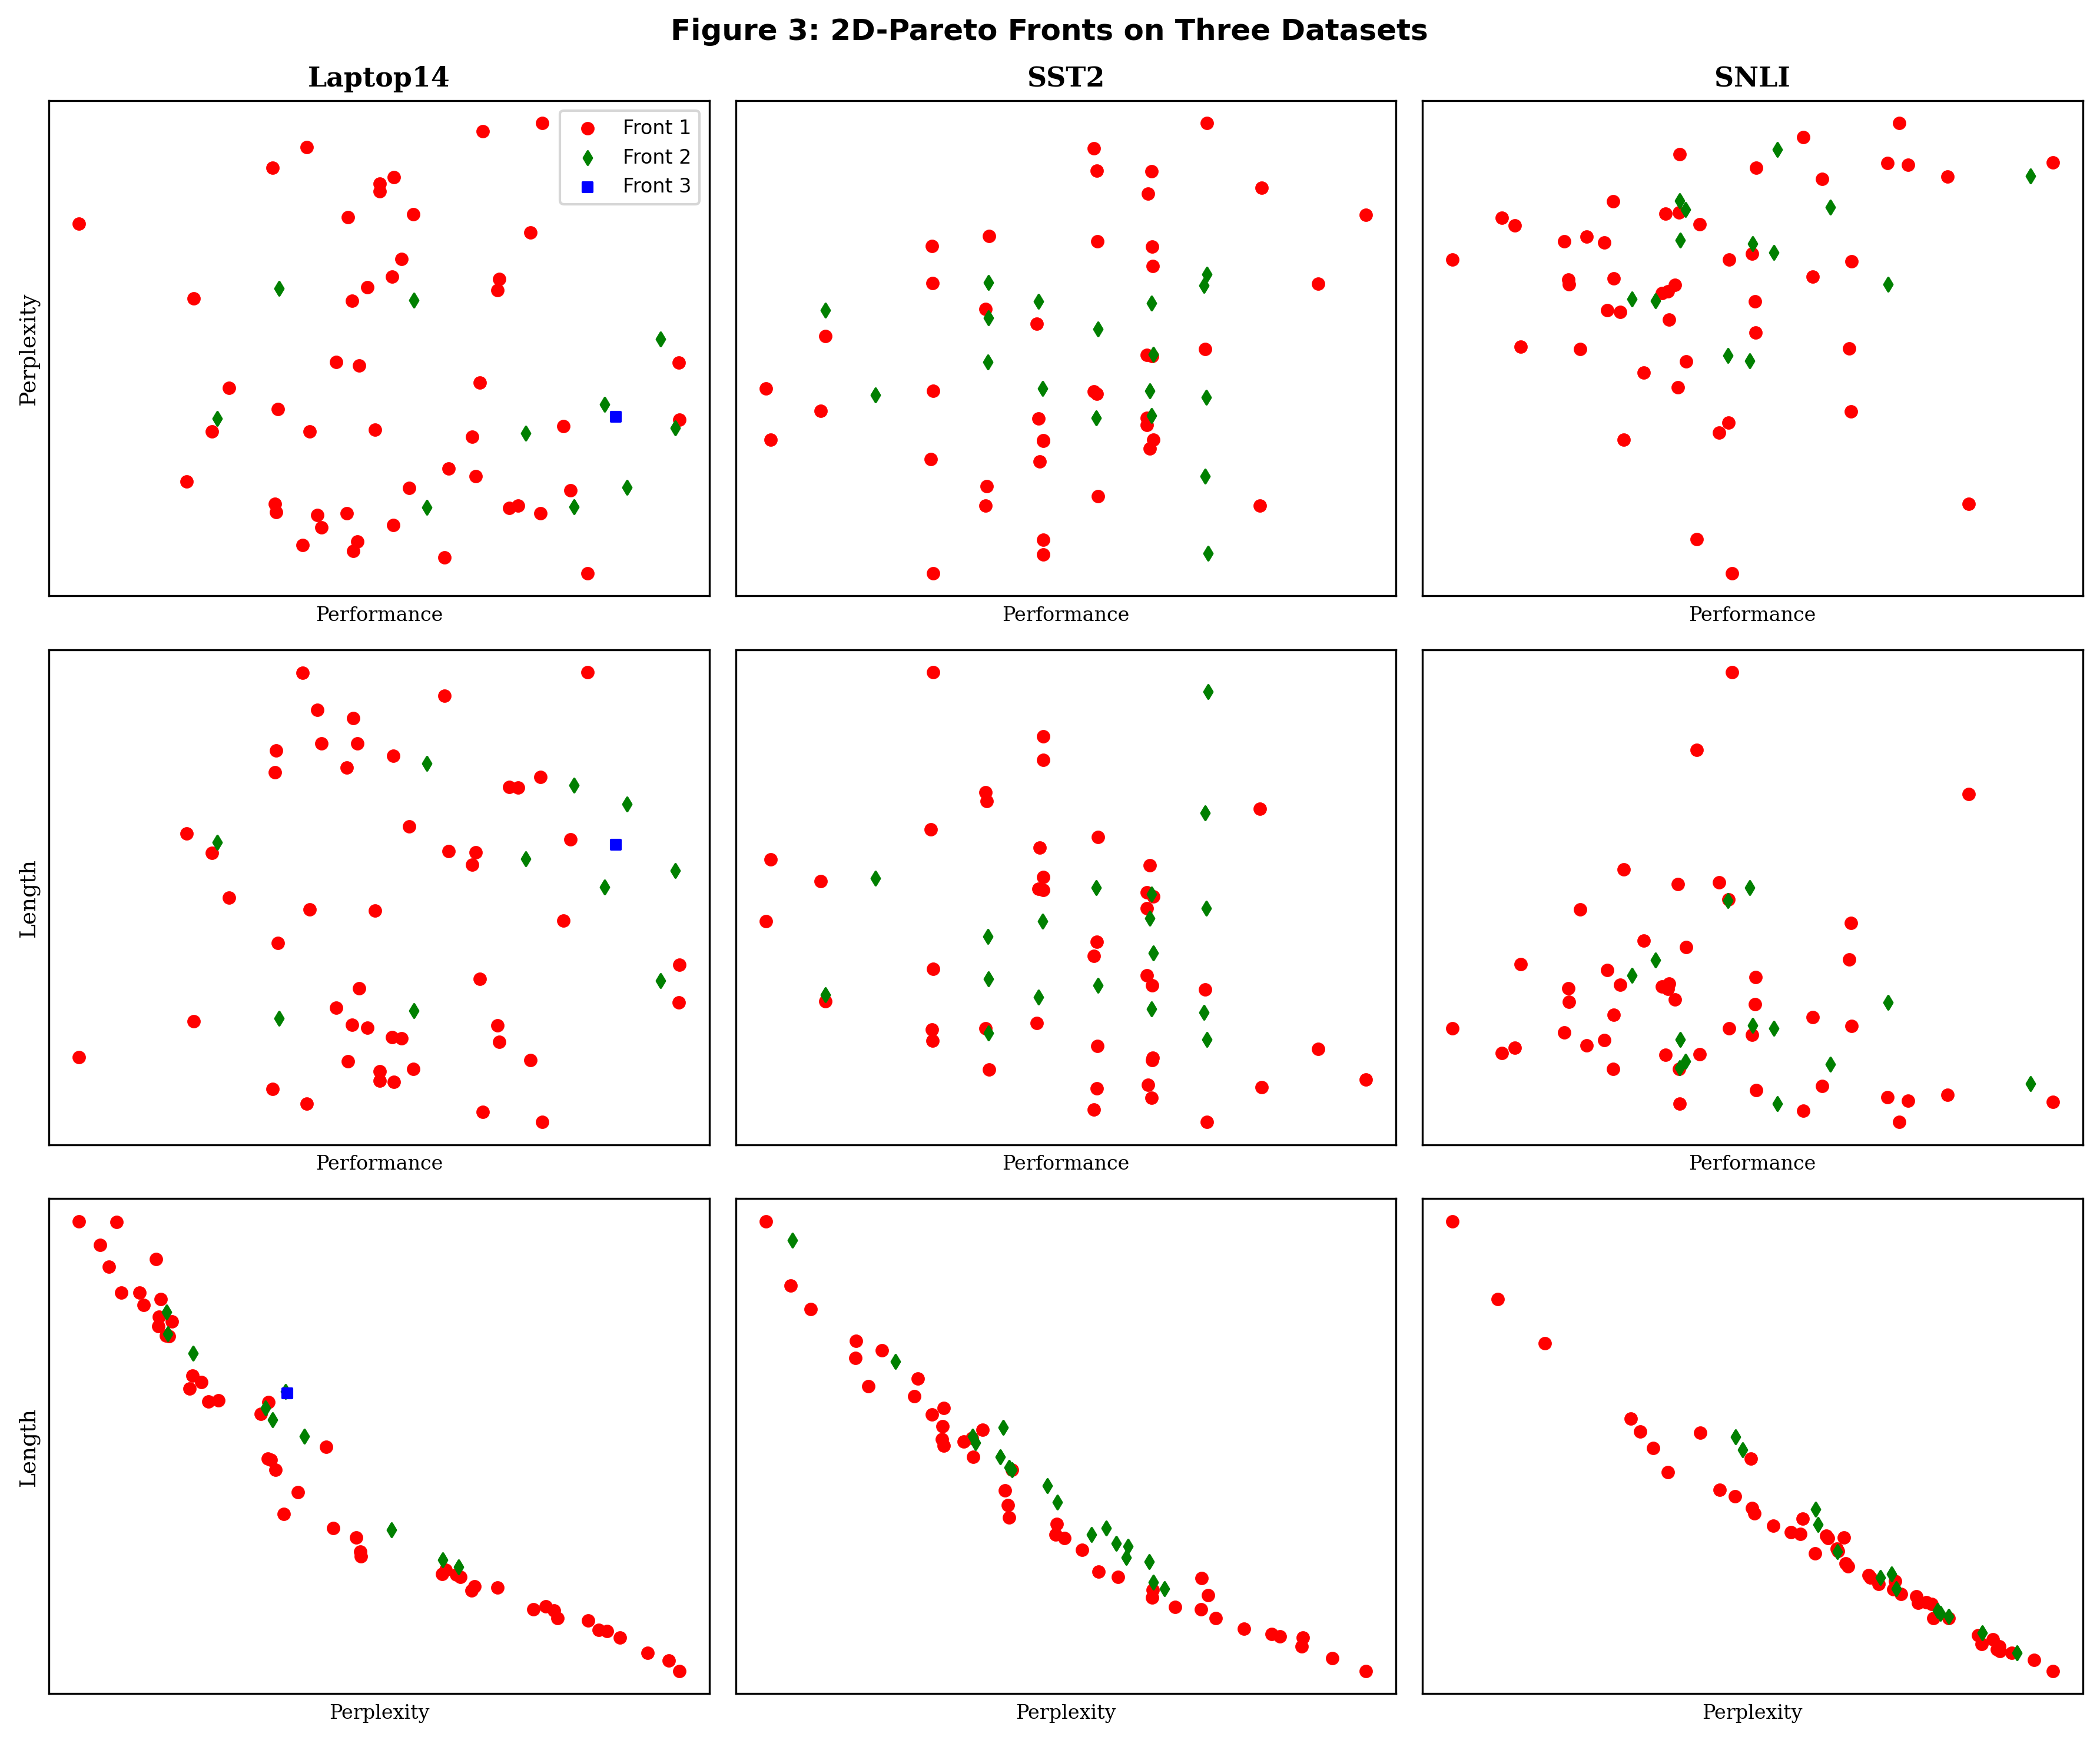
\includegraphics[width=\textwidth, height=0.75\textheight, keepaspectratio]{paper_fig3_pareto.png}
\end{figure}
\end{frame}

\begin{frame}{Pareto Front}
    \begin{block}{Kết luận}
        Pareto front đa dạng cho phép người dùng lựa chọn instruction phù hợp với ràng buộc tài nguyên (ưu tiên ngắn gọn, dễ hiểu hay hiệu suất cao) -- điều mà single-objective optimization không thể cung cấp.
    \end{block}
\end{frame}

%--------------------------------------------------------
% LIMITATIONS SECTION
%--------------------------------------------------------
\section{Hạn chế}

\begin{frame}{Mục lục}
    \setbeamercovered{dynamic}
    \tableofcontents[currentsection]
\end{frame}

\begin{frame}{Hạn chế}
    \begin{block}{1. Nguy cơ hội tụ tại cực trị cục bộ}
        \textbf{Nguyên nhân:} InstOptima khởi đầu từ các instruction được tạo thủ công. \\
        \textbf{Vấn đề:}
        \begin{itemize}
            \item Khởi tạo kém có thể làm lệch hướng tìm kiếm vĩnh viễn.
            \item Quá trình tiến hóa có thể bị mắc kẹt và hội tụ về vùng nghiệm dưới tối ưu.
        \end{itemize}
    \end{block}
\end{frame}

\begin{frame}{Hạn chế}
    \begin{block}{2. Chi phí tính toán cao}
        \textbf{Nguyên nhân:} Mỗi thế hệ đòi hỏi gọi LLM API, đánh giá đầy đủ ba mục tiêu và lặp lại việc inference/fine-tuning mô hình. \\
        \textbf{Vấn đề:}
        \begin{itemize}
            \item Thời gian chạy và chi phí tài chính rất lớn.
        \end{itemize}
    \end{block}
\end{frame}

\section{Demo}
\begin{frame}{Mục lục}
    \setbeamercovered{dynamic}
    \tableofcontents[currentsection]
\end{frame}

\begin{frame}
\begin{center}
\Large{\textbf{Cảm ơn thầy đã lắng nghe!}}
\end{center}
\end{frame}

\end{document}
